%% LyX 2.0.2 created this file.  For more info, see http://www.lyx.org/.
%% Do not edit unless you really know what you are doing.
\documentclass[english]{article}
\usepackage[T1]{fontenc}
\usepackage[latin9]{inputenc}
\usepackage{geometry}
\geometry{verbose,tmargin=2cm,bmargin=2.5cm}
\usepackage{float}
\usepackage{amsthm}
\usepackage{amsmath}
\usepackage{graphicx}

\makeatletter
%%%%%%%%%%%%%%%%%%%%%%%%%%%%%% Textclass specific LaTeX commands.
\numberwithin{equation}{section}
\numberwithin{figure}{section}

%%%%%%%%%%%%%%%%%%%%%%%%%%%%%% User specified LaTeX commands.
\date{}

\makeatother

\usepackage{babel}
\begin{document}

\title{How to make a movie using VisIt }


\author{Yiyang Yang}


\date{May 2014}

\maketitle
VisIt is a free, open source, platform independent, parallel visualization
toll for visualing data defined on two- and three-dimensional structured
and unstructured meshes. This manual shows how to use VisIt to make
an animated movie with the \emph{vtk} files generated by \emph{FronTier++}.


\subsection*{Step 1: Opening a file}
\begin{itemize}
\item VisIt can be started by typing \emph{visit} at the prompt as Figure
0.1 and the first thing is to open files with suffix \emph{.visit}
generated by \emph{FronTier++}.
\begin{figure}[H]
\begin{centering}
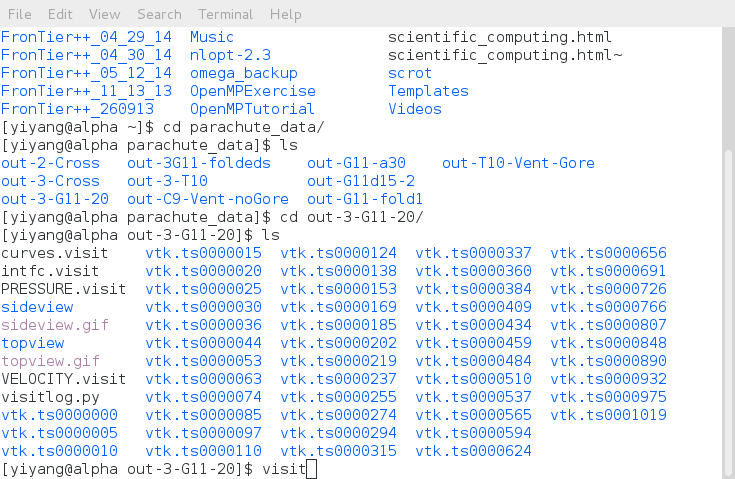
\includegraphics[scale=0.4]{scrot/visit_01}
\par\end{centering}

\caption{run the software}
\end{figure}

\item Select a file by clicking \emph{Open} on the left panel as shown in
Figure 0.2.
\begin{figure}[H]
\centering{}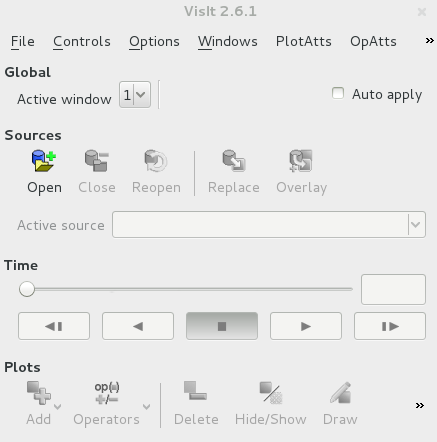
\includegraphics[scale=0.4]{scrot/visit_02}\caption{open \emph{.visit} file}
\end{figure}

\item The window in Figure 0.3 will pop up and choose the objective file,
in this case \emph{curves.visit}, then click \emph{OK}. You can change
the directory through\emph{ Path }or the left subwindow\emph{ Directories.}
\begin{figure}[H]
\begin{centering}
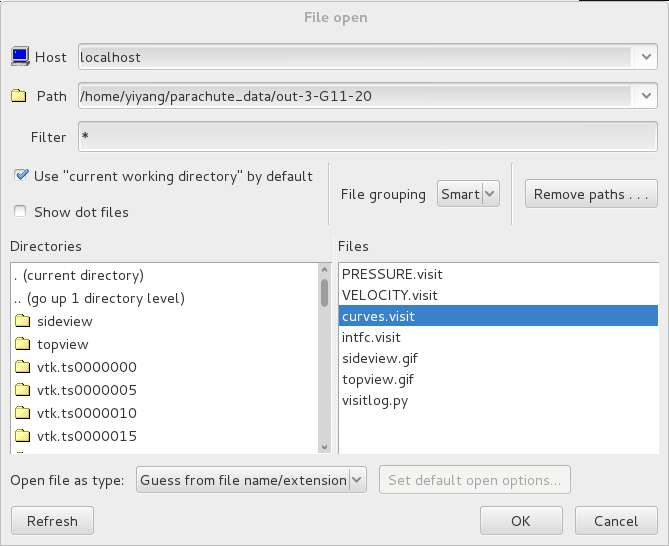
\includegraphics[scale=0.4]{scrot/visit_03}
\par\end{centering}

\caption{open \emph{.visit} file (cont.)}
\end{figure}

\item With the same steps, you can open other files in the directory, such
as \emph{intfc.visit, VELOCITY.visit} etc and they will all be available
in the pulldown menu of \emph{Active source}.
\end{itemize}

\subsection*{Step 2: Creating a plot}
\begin{itemize}
\item To create a plot with the active source, click \emph{Add} in the subwindow
\emph{Plots}. 
\begin{figure}[H]
\begin{centering}
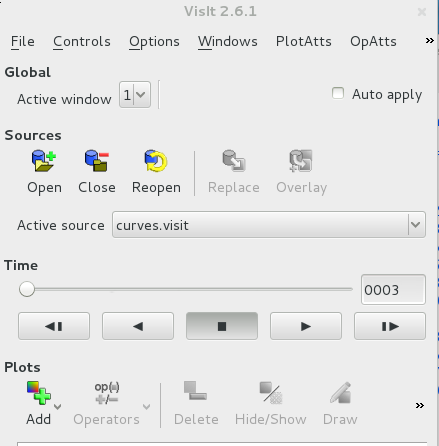
\includegraphics[scale=0.4]{scrot/visit_04}
\par\end{centering}

\caption{create a plot}
\end{figure}

\item In the pulldown menu of \emph{Add}, choose \emph{mesh}, then \emph{mesh}.
In this way, the data of \emph{curves.visit} is ready to plot in the
form of mesh.
\begin{figure}[H]
\begin{centering}
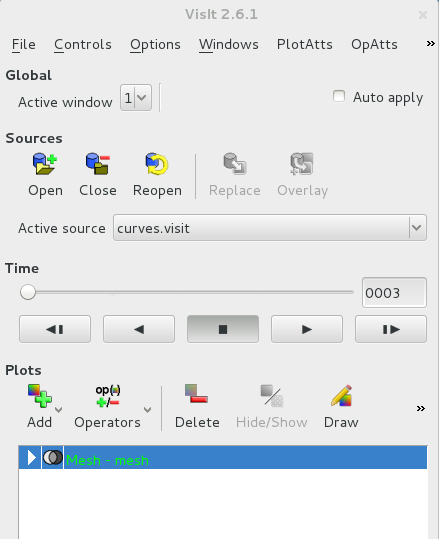
\includegraphics[scale=0.4]{scrot/visit_05}
\par\end{centering}

\caption{create a plot (cont.)}


\end{figure}

\item To add the data of interface, change the \emph{Active source} to \emph{intfc.visit};
click \emph{Add} and choose \emph{Pseudocolor}, then \emph{jacobian}.
Meanwhile, a window as shown in Figure 0.6 will pop up asking about
correlation between current data and previous data. Click \emph{YES}
to make them correlated in time. In this way, the data in \emph{intfc.visit}
is added in the form of Pseudocolor and is related with the data in
\emph{curves.visit}. 
\begin{figure}[H]
\begin{centering}
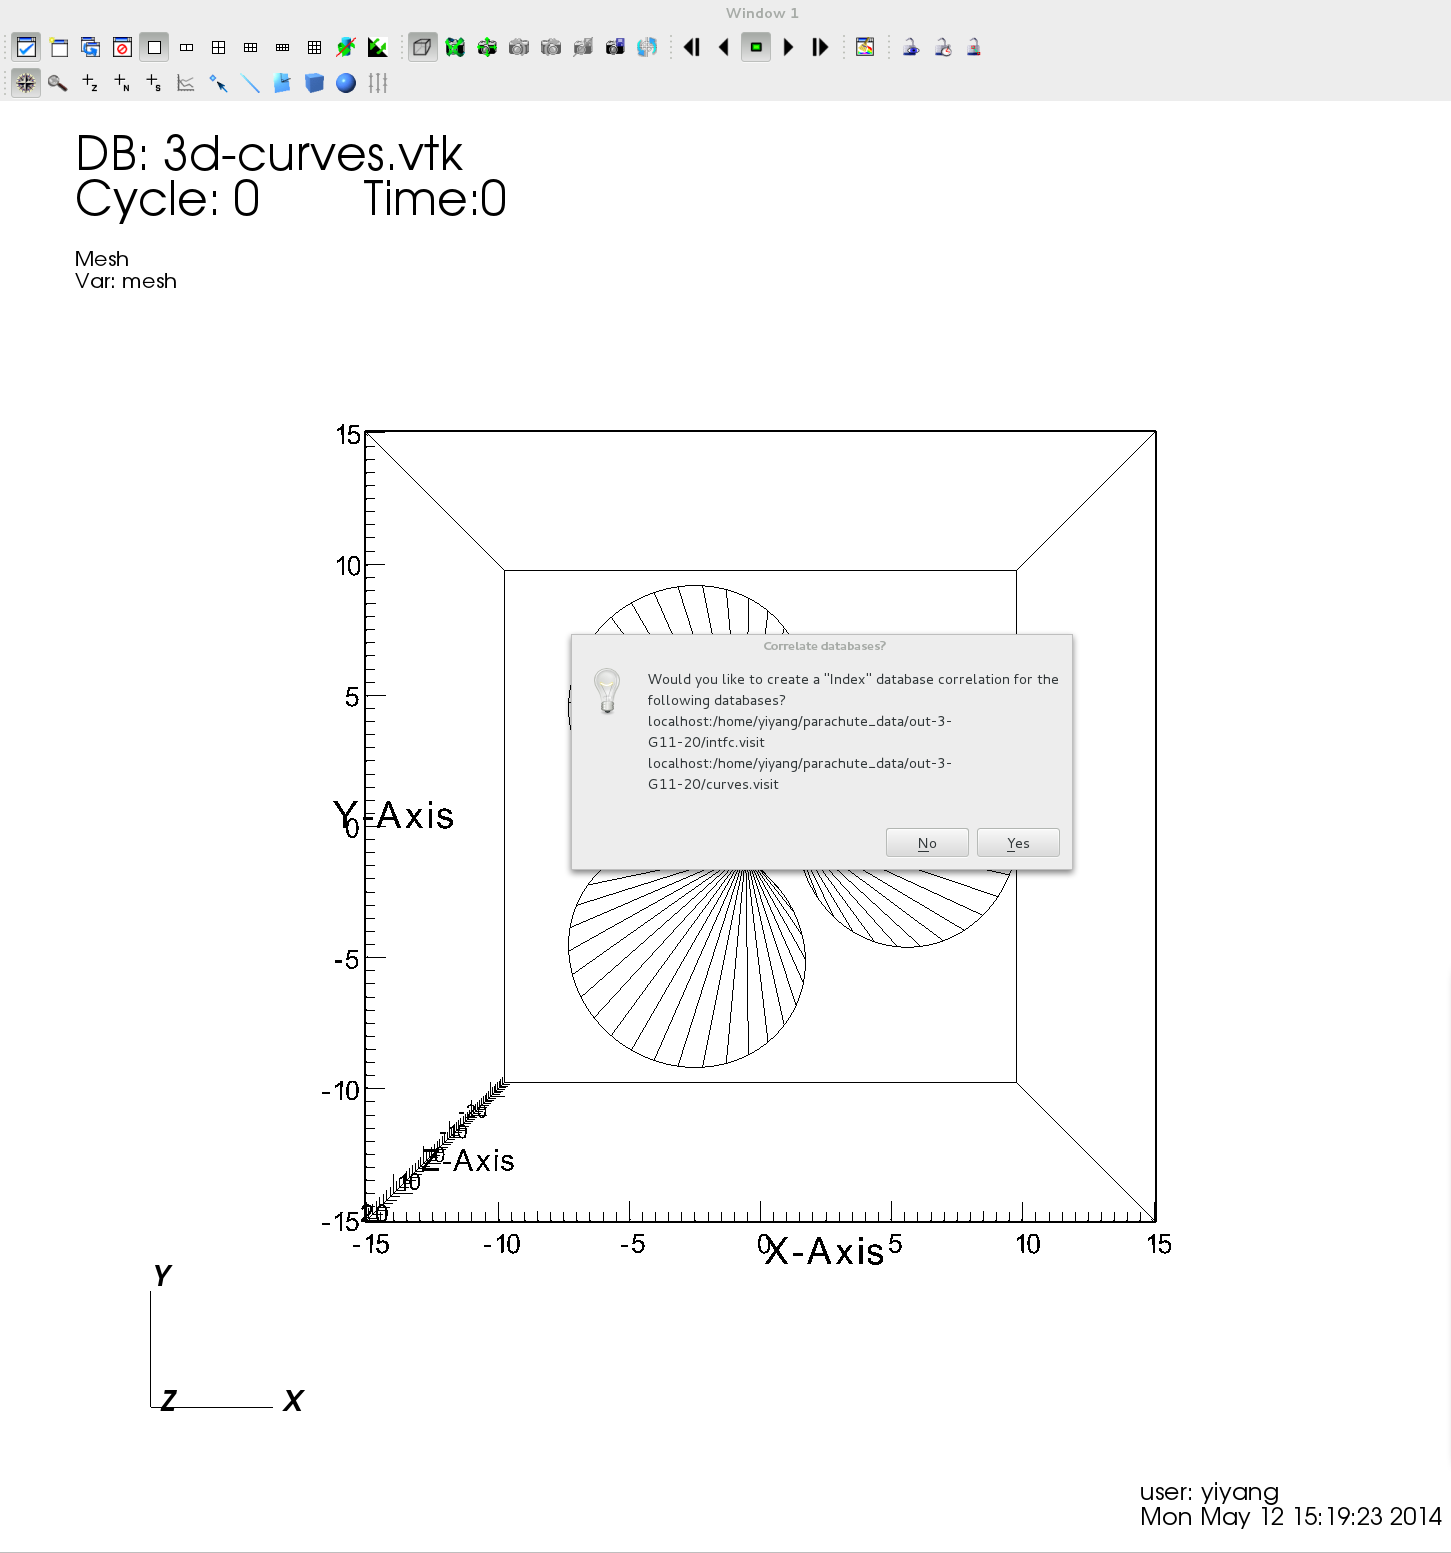
\includegraphics[scale=0.2]{scrot/visit_06}
\par\end{centering}

\caption{create a plot (cont.)}
\end{figure}

\item Click \emph{Draw} in \emph{Plots} panel to create a plot. The detail
of Pseudocolor can be altered through the \emph{Pseudocolor plot attributes}
panel which can be accessed by double clicking \emph{Pseudocolor}
in main window. 
\begin{figure}[H]
\begin{centering}
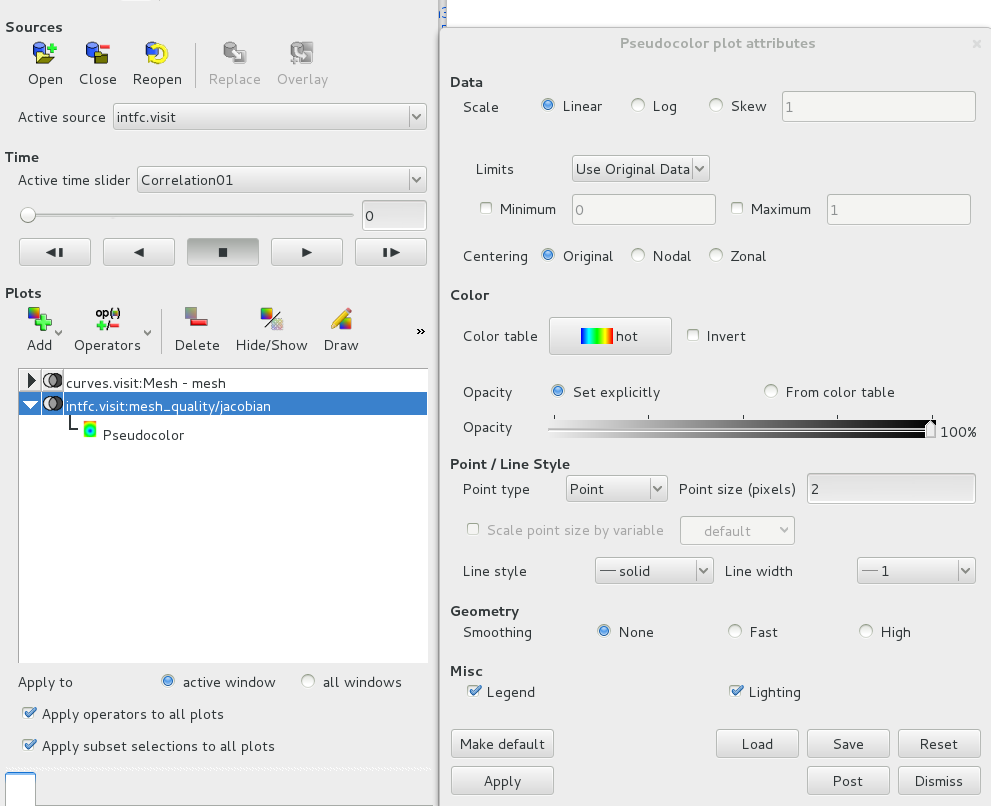
\includegraphics[scale=0.2]{scrot/visit_07}
\par\end{centering}

\caption{change Pseudocolor setting}
\end{figure}

\item The buttons in Figure 0.8 can adjust location and size of the plot.
\begin{figure}[H]
\begin{centering}

\includegraphics[scale=0.4]{scrot/visit_08}
\par\end{centering}

\caption{adjust location and size}
\end{figure}

\item The buttons in Figure 0.9 can adjust viewing angle of the plot.
\begin{figure}[H]
\begin{centering}

\includegraphics[scale=0.4]{scrot/visit_09}
\par\end{centering}

\caption{adjust viewing angle}


\end{figure}

\end{itemize}

\subsection*{Step 3: Saving a movie}
\begin{itemize}
\item In the pulldown menu of \emph{File}, click \emph{save movie}. Following
window will pop up, choose \emph{New simple movie}, then click \emph{Next}.
\begin{figure}[H]
\begin{centering}
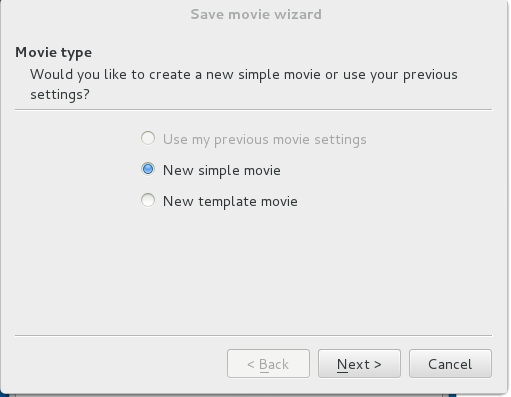
\includegraphics[scale=0.4]{scrot/visit_10}
\par\end{centering}

\caption{save a movie}
\end{figure}

\item Change \emph{Format} to \emph{JPEG images}, specify \emph{window size},
add them to \emph{Output}, then click \emph{Next}. 
\begin{figure}[H]
\begin{centering}
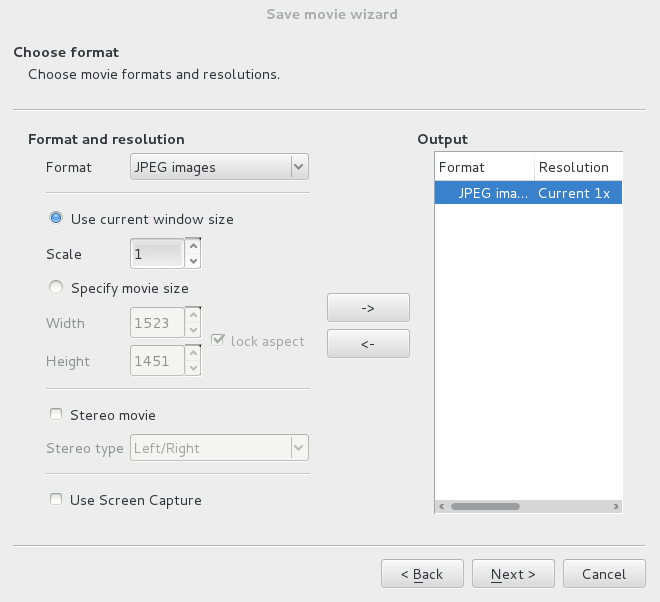
\includegraphics[scale=0.4]{scrot/visit_11}
\par\end{centering}

\caption{save a movie (cont.)}
\end{figure}

\item In the window shown as Figure 0.12, click \emph{Next}.
\begin{figure}[H]
\begin{centering}
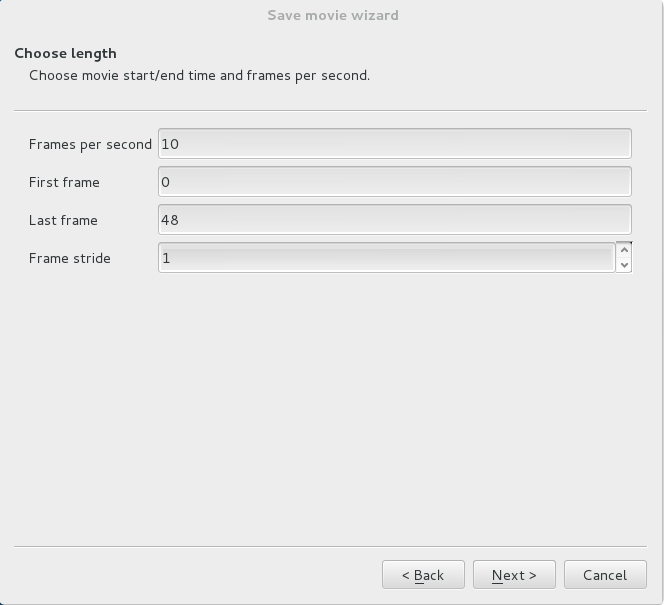
\includegraphics[scale=0.4]{scrot/visit_12}
\par\end{centering}

\caption{}
\end{figure}

\item Set a \emph{Base filename} which will be the prefix of the generated
.jpeg images, then click \emph{Next}.
\begin{figure}[H]
\begin{centering}
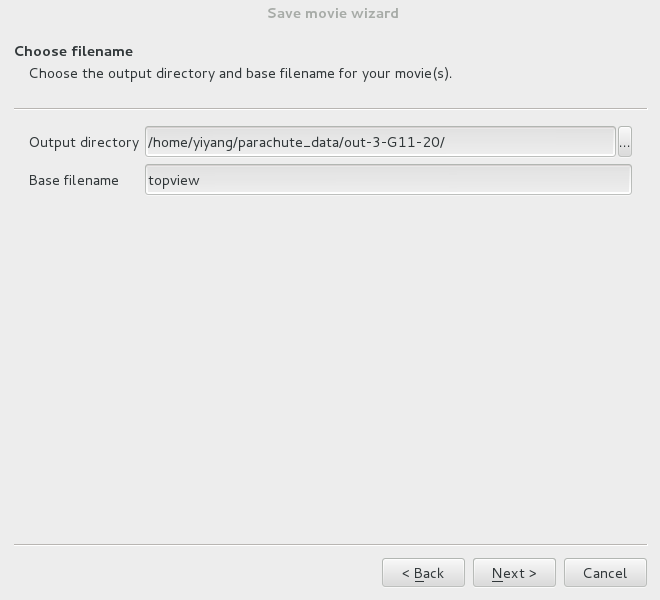
\includegraphics[scale=0.4]{scrot/visit_13}
\par\end{centering}

\caption{save a movie (cont.)}
\end{figure}

\item In the following window, click Next. 
\begin{figure}[H]
\begin{centering}
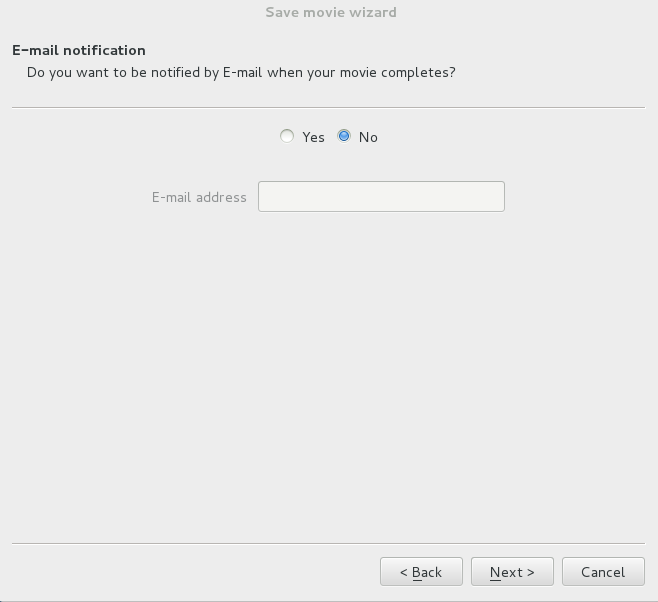
\includegraphics[scale=0.4]{scrot/visit_14}
\par\end{centering}

\caption{save a movie (cont.)}


\end{figure}

\item Click \emph{Finish}.
\begin{figure}[H]
\begin{centering}
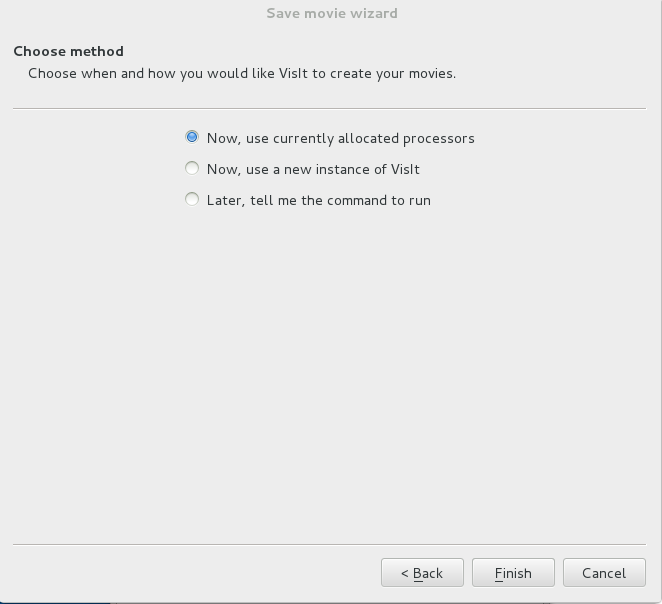
\includegraphics[scale=0.4]{scrot/visit_15}
\par\end{centering}

\caption{save a movie (cont.)}
\end{figure}

\item Figure 0.16 shows the saving process.
\begin{figure}[H]
\begin{centering}
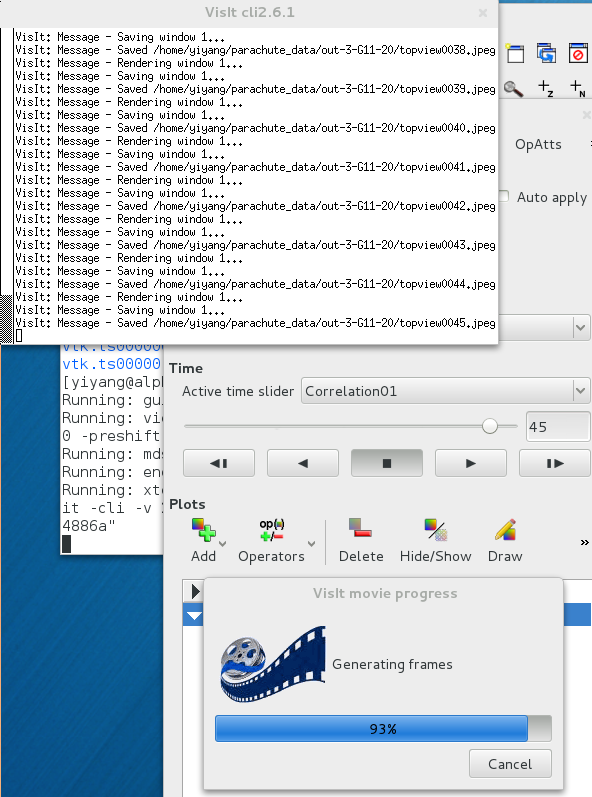
\includegraphics[scale=0.2]{scrot/visit_16}
\par\end{centering}

\caption{save a movie (cont.)}
\end{figure}

\item Convert generated images topview00{*}.jpeg into animation topview.gif
with command: \emph{convert topview00{*}.jpeg topview.gif}.
\begin{figure}[H]
\begin{centering}
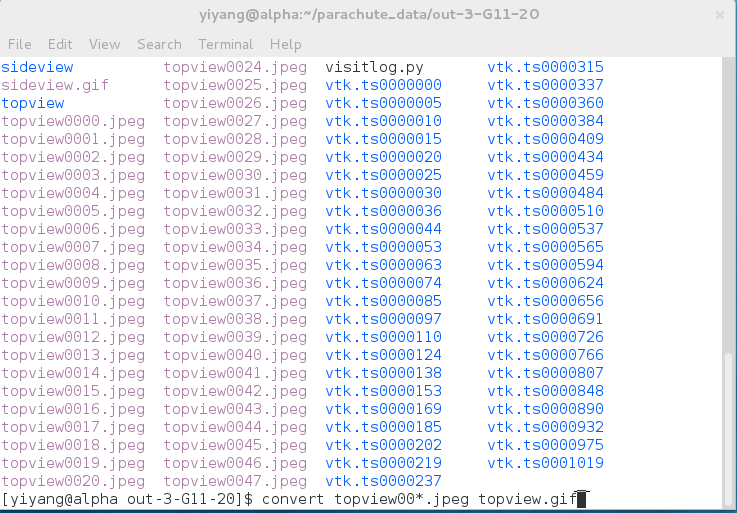
\includegraphics[scale=0.4]{scrot/visit_17}
\par\end{centering}

\caption{generate a movie}
\end{figure}

\item Play the movie topview.gif with command: \emph{animate topview.gif}.
\begin{figure}[H]
\begin{centering}
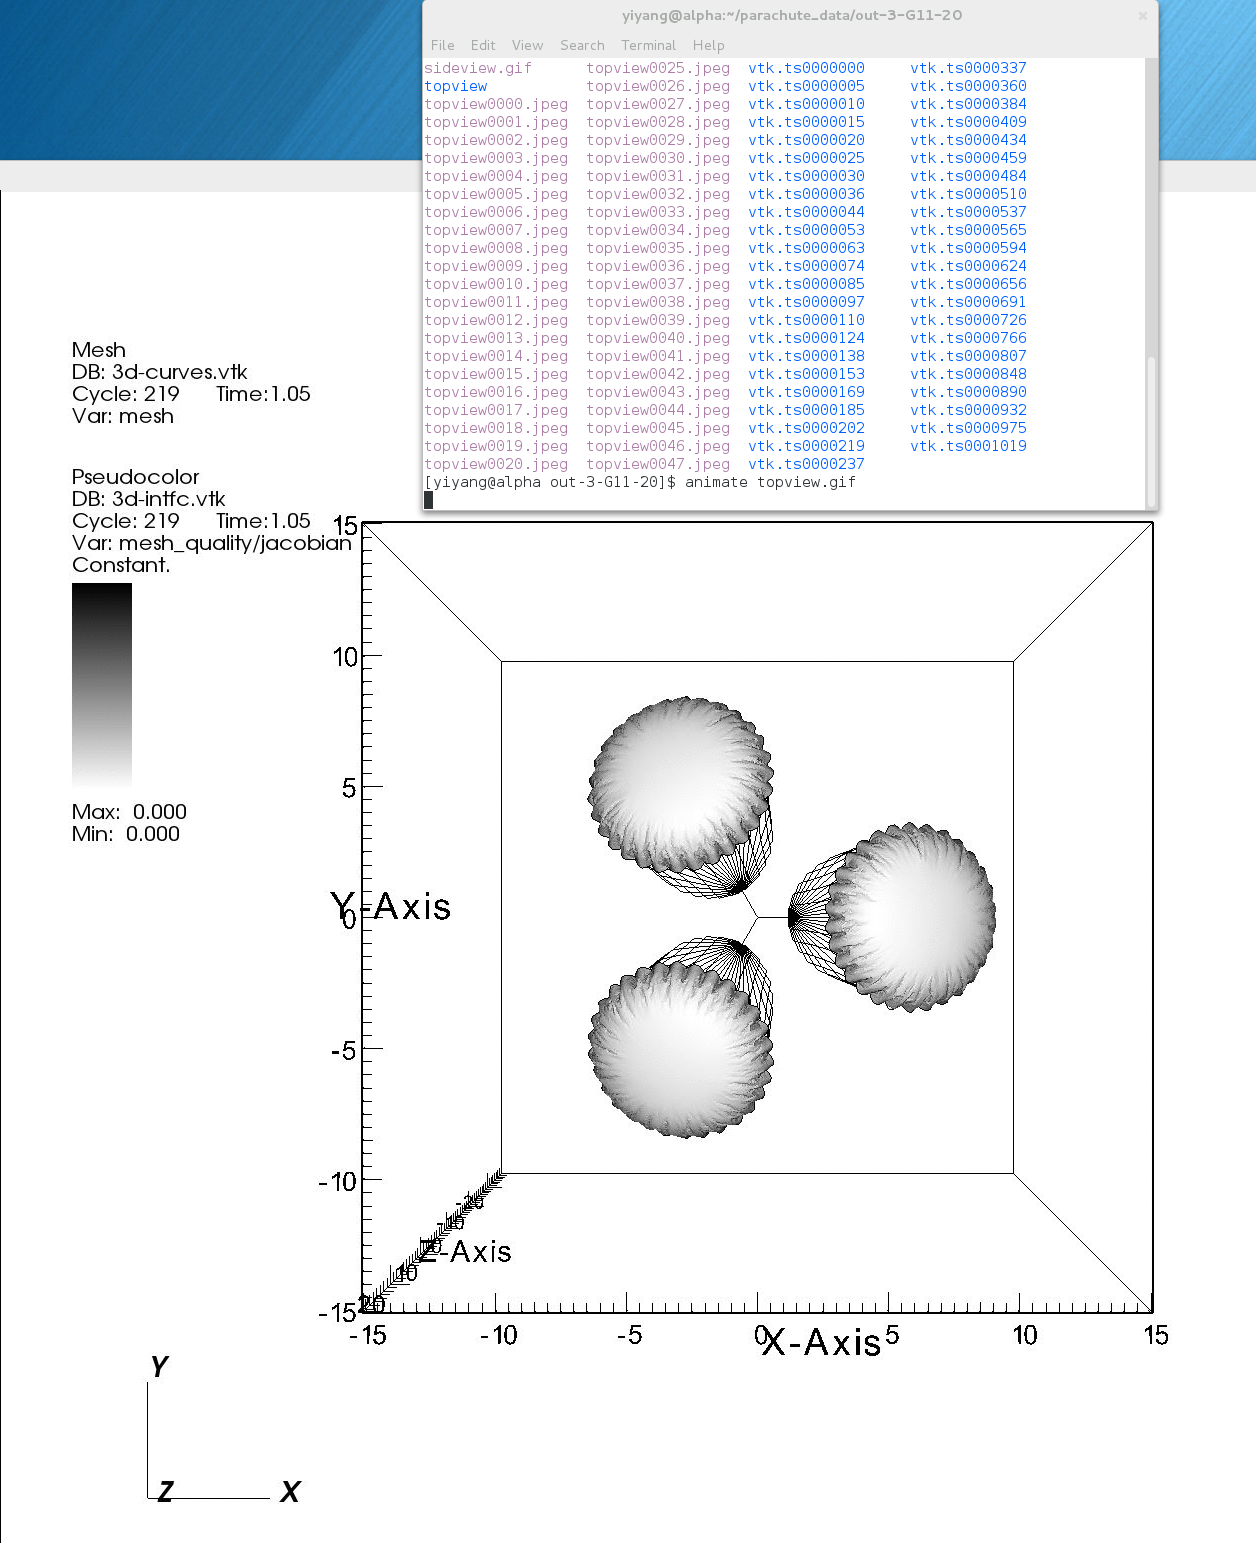
\includegraphics[scale=0.2]{scrot/visit_18}
\par\end{centering}

\caption{diaplay a movie}


\end{figure}
\end{itemize}

\end{document}
